\documentclass[colorlinks,10pt]{beamer}
% compress
%\documentclass[handout,xcolot=pdftex,dvipsnames,table]{beamer}
%\definecolor{mybg}{RGB}{255,255,204}
\definecolor{mybg}{RGB}{238,255,170}


\usepackage{graphicx}
\usepackage{color}

\mode<presentation>
\setbeamercovered{invisible}
\usetheme{Warsaw}
\usecolortheme{dolphin}

\usefonttheme{serif}



\usepackage[spanish]{babel}
\usepackage[utf8]{inputenc}
\usepackage{amsmath}
\usepackage{relsize}
\usepackage{hyperref}
\usepackage{alltt}



\usepackage{times}
\usepackage[square, sort, numbers, authoryear]{natbib}
\bibliographystyle{plainnat}

\usepackage{beamerthemesplit}
%\usetheme{Berkeley}
%\usecolortheme{dolphin}





% Delete this, if you do not want the table of contents to pop up at
% the beginning of each subsection:
\AtBeginSection[]
{
\begin{frame}<beamer>{Outline}
\tableofcontents[currentsection]
\end{frame}
}
\title{ Python para RPi}
\subtitle
 {Parte I:  Introducción a GNU/Linux y Python} % (optional)

\author[Velasco and Perera]{Manel Velasco,\inst{1} PhD and Alexandre Perera,\inst{1}$^{,}$\inst{2} PhD}

\institute[UPC] % (optional, but mostly needed)
{
  \inst{1}%
  Departament d'Enginyeria de Sistemes, Automatica i Informatica Industrial (ESAII)  \\
  Universitat Politecnica de Catalunya 
  \and 
  \inst{2}%
   Centro de Investigacion Biomedica en Red en Bioingenieria, Biomateriales y Nanomedicina (CIBER-BBN)  \\
    \href{mailto:Alexandre.Perera@upc.edu}{Alexandre.Perera@upc.edu}~\href{mailto:manel.velasco@upc.edu}{Manel.Velasco@upc.edu}
}
 

\date[Feb, 2013, Learning Python]{Introduction to Python for Engineering and Statistics\\
Febraury, 2013}

 %





\mode<presentation>
\setbeamercovered{invisible}
\usetheme{Warsaw}
\usecolortheme{dolphin}
\usefonttheme{serif}



\begin{document}



\begin{frame}[plain]
   %  \titlepage
   \maketitle
\end{frame}


\section{Content}



\begin{frame}
  \setbeamercovered{dynamic}
  \frametitle{ Introducción al curso}
  Este curso se estructura en cinco partes: 
  \begin{enumerate}
  \item Introducción a GNU/Linux
  \item Python
  \item Raspberry Pi
  \item Python en la Raspberry Pi
  \end{enumerate}

\end{frame}

\section{Sobre los Autores}
\begin{frame}[shrink]\frametitle{Scipy Lecture Notes}
    \small Algunas partes de este seminario contiene material de \href{http://scipy-lectures.github.com/}{http://scipy-lectures.github.com's Scipy Lecture Notes}. Esta web es un proyecto de código abierto para la creación de material para la enseñanza de python, incluyendo teoría, ejercicios y herramientas.

    \Tiny
\begin{columns}[c]
\column{0.5\textwidth}
\begin{block}{Editors}
\begin{itemize}
    \item Valentin Haenel
    \item Emmanuelle Gouillart
    \item  Gaël Varoquaux
\end{itemize}          
\end{block}
\begin{block}{Additional Contributors}

    \begin{itemize}  
        \item  Akihiro Uchida
        \item Corey Farwell
        \item egens
        \item Lars Buitinck
        \item  Olivier Verdier
        \item Virgile Fritsch
    \end{itemize}
\end{block}

\column{0.5\textwidth}
\begin{block}{Authors}
\begin{itemize}
    \item  Christopher Burns
    \item Adrian Chauve
    \item Robert Cimrman
    \item Christophe Combelles
    \item André Espaze
    \item Emmanuelle Gouillart
    \item Mike Müller
    \item Fabian Pedregosa
    \item Didrik Pinte
    \item Nicolas Rougier
    \item Gaël Varoquaux
    \item Pauli Virtanen
    \item Zbigniew Jedrzejewski-Szmek
\end{itemize}
\end{block}
\end{columns}

\end{frame}



%----------------------------FRAME 2 cols + header (box)-------------
\begin{frame}[plain]\frametitle{About Us}
\begin{block}{Manel Velasco, PhD}
    \small Manel Velasco graduated in maritime engineering in 1999 and received the PhD degree in automatic control in 2006, both from the Technical University of Catalonia, Barcelona, Spain.  He has been involved in research on artificial intelligence from 1999 to 2002 and, since 2000, on the impact of real-time systems on control systems. His research interests include artificial intelligence, real-time control systems, and collaborative control systems, especially on redundant controllers and multiple controllers with self-interacting systems.
\end{block}

    \begin{columns}[c]
\column{0.65\textwidth}

Automatic Control Department\\
Universitat Politècnica de Catalunya\\
Pau Gargallo, 5\\
08028 Barcelona (Spain)\\
Phone: +34 93 401 1681\\
Fax: +34 93 401 7045\\
\href{manel.velasco@upc.edu}{manel.velasco@upc.edu}
\column{0.35\textwidth}
\begin{figure}[!htb]
    \centering
    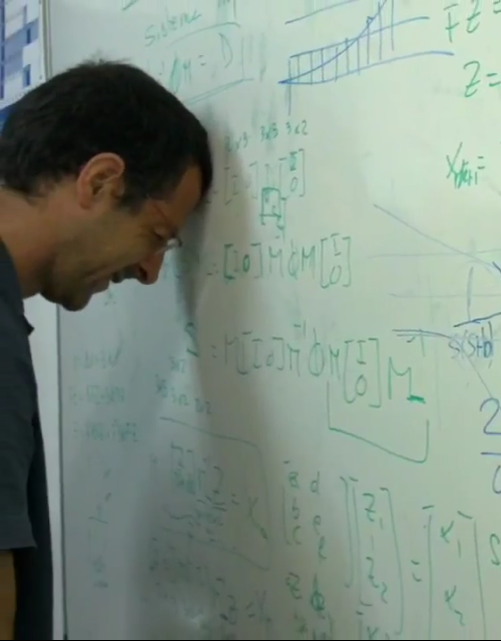
\includegraphics[width=\textwidth]{figs/manel}
\end{figure}
\end{columns}
\end{frame}


%----------------------------FRAME 2 cols + header (box)-------------
\begin{frame}[plain]\frametitle{About Us}

\begin{block}{Alexandre Perera, PhD}

    \small Alexandre Perera-LLuna graduated in physics at University of Barcelona at 1999 and in electrical engineering at 2001, he received a PhD degree in physics from the same university in 2003. He stayed as a postdoctoral fellow at Texas A\&M University (USA) and in Universitat Politècnica de Catalunya(Spain) as a Ramon y Cajal Fellow from 2008-1012. His main area of expertise covers machine learning, statistical analysis, and data mining in biomedical systems, bioengineering and bioinformatics. He is an Associate Professor at Universitat Politècnica de Catalunya-BarcelonaTech (UPC).
\end{block}
\begin{columns}[c]
\column{0.65\textwidth}
Automatic Control Department\\
Universitat Politècnica de Catalunya\\
Pau Gargallo, 5\\
08028 Barcelona (Spain)\\
Phone: +34 93 401 6963\\
Fax: +34 93 401 7045\\
\href{Alexandre.Perera@upc.edu}{Alexandre.Perera@upc.edu}

 
\column{0.35\textwidth}
\begin{figure}[!htb]
    \centering
    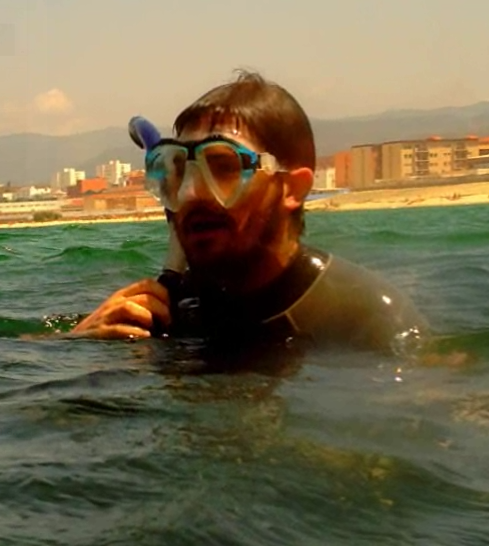
\includegraphics[width=\textwidth]{figs/alex1}
\end{figure}
\end{columns}
\end{frame}



% section Preparation (end)
%----------------------------FRAME------------------------------------
\begin{frame}[fragile]\frametitle{About this course}
\begin{block}{}


    \begin{itemize}
        \item Todo el material se ha preparado empleando \LaTeX~ y ediado en  \href{http://www.vim.org}{Vim} (por desgracia de  Alex).
        \item El código Python están empotrados en  \LaTeX con la ayuda de  \href{http://mpastell.com/pweave/}{Pweave}, desarrollado por  Matti Pastell. 
        \item Todo el código Python se ha marcado en el documento mediante el paquete  \emph{minted}, desarrollado por Konrad Rudolph, el \emph{python syntax highlighter} \href{http://pygments.org}{Pygments}, y código bash propio. 
    \end{itemize}
    \end{block}

\end{frame}


\section{Introducción a GNU/Linux}

\subsection{Porqué GNU/Linux ?}


\begin{frame}
  \frametitle{Uso de los sistemas operativos de escritorio}
  
  \begin{center}
    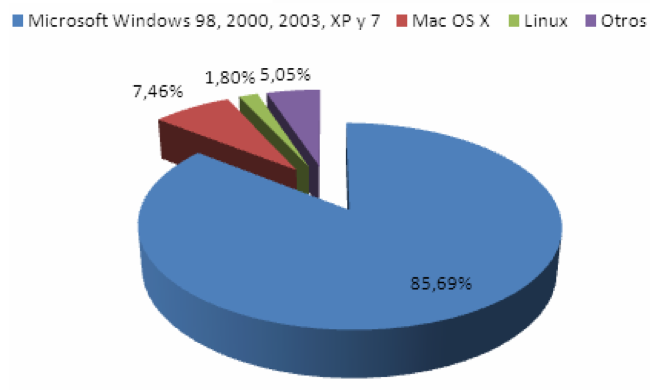
\includegraphics[width=0.8\textwidth]{figs/SOSdesktop}
  \end{center}
\end{frame}



\begin{frame}
  \frametitle{Sistemes operatius més usats en mòbils}
  Aunque no es estrictamente cierto....
  \pause \begin{center}
    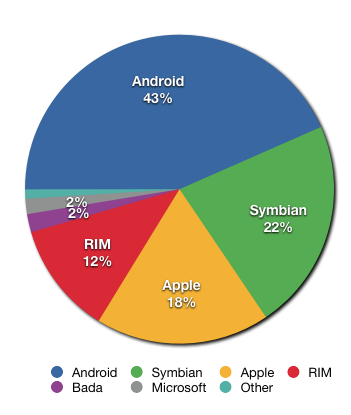
\includegraphics[width=0.6\textwidth]{figs/Smartphone_share_current} \\
  \end{center}
%  \small{ extret de: \href{http://news.netcraft.com/whats/}{http://news.netcraft.com/}}
\end{frame}


\begin{frame}
  \frametitle{Android}
  
  \begin{columns}
    \begin{column}{0.6\textwidth}
      \begin{block}{Android es...}
        Un conjunto de programas para teléfonos mobiles, que incluye un sistema operativo y un conjunto de librerías y aplicaciones.\\
        En 2005, Google Inc. compró Android a Android Inc. Android se basa en una versión modificada del kernel de Linux\\ 
        Android Open Source Project (AOSP) tiene como objetivo mantener y desarrollar el sistema operativo Android. Android es la plataforma de sistemas móbiles con más prevalente. 
      \end{block}
    \end{column}
    \begin{column}{0.4\textwidth}
        \begin{center}
    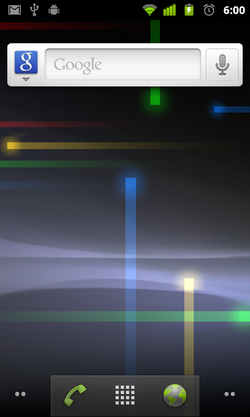
\includegraphics[width=0.9\columnwidth]{figs/android} \\
  \end{center}
    \end{column}
  \end{columns}
\end{frame}




\begin{frame}
  \frametitle{iOS (iphone)}
  
  \begin{columns}
    \begin{column}{0.6\textwidth}
      \begin{block}{Android és...}
        iOS es el sistema operativo del iPhone, iPod Touch, iPad, que es el mismo sistema operativo que el sistema de escritorio de Mac, OS X. \\
        Mac OS X es una versión del sistema operativo que utilizan los ordenadores Macintosh, basados en un sistema operativo UNIX. 
      \end{block}
    \end{column}
    \begin{column}{0.4\textwidth}
        \begin{center}
    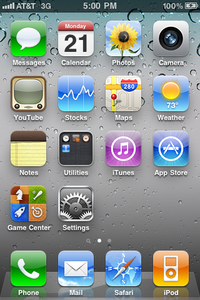
\includegraphics[width=0.9\columnwidth]{figs/ios} \\
  \end{center}
    \end{column}
  \end{columns}
\end{frame}




\begin{frame}
  \frametitle{Usos de UNIX y GNU/Linux}
  \begin{block}{Linux se usa en:}
    \begin{itemize}
    \item U.S. Department of Defense
    \item  Parlamento Francés
    \item Google
    \item IBM
    \item E*Trade (La bolsa de Nova York)
    \item Servidores de Bases de Datos
    \item Maquinaria industrial
    \item Routers ADSL
    \item \textcolor{blue}{61\% de los Teléfonos móviles !!}
    \end{itemize}
  \end{block}
 \pause 
 \begin{block}{y en ....}
   La Raspberry Pi !!
 \end{block}
\end{frame}



% Potser posar a la historia de unix
\begin{frame}
  \frametitle{Historia de GNU/Linux y UNIX}
  \pause \begin{center}
    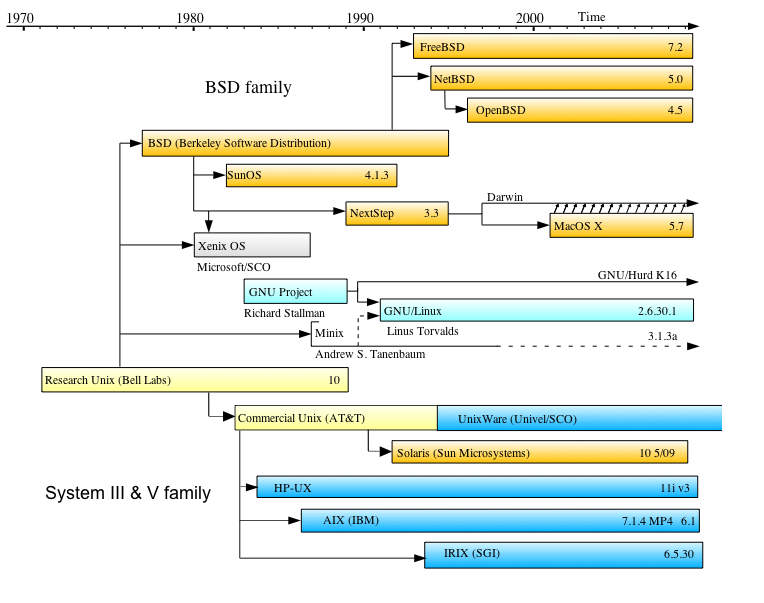
\includegraphics[width=0.9\textwidth]{figs/unixhistory} \\
  \end{center}
%  \small{ extret de: \href{http://news.netcraft.com/whats/}{http://news.netcraft.com/}}
\end{frame}




\begin{frame}
  \frametitle{Propiedades de GNU/Linux} 
  
  \begin{itemize}
  \item<+-> Un sistema operativo de 32/64 bits clon de UNIX
  \item<+-> Herramientas para la gestión avanzada y no interactiva de un sistema  (sed, awk, bash, grep, etc)
    
  
  \item<+-> Compiladores: C, C++, Fortran, Ada, etc
  \item<+-> Interpretes: \emph{Python}, java, R, octave, etc
  

  \item<+->  Multi-usuario, multi-tarea, multi-processador
  \item<+->  Puede coexistir con otros sistemas  operativos (grub)
  \item<+->  Corre en diferentes plataformas (móviles, Raspberry Pi)
  \item<+->  Su código fuente es abierto, libre y pertenece a la comunidad. 
  \end{itemize}
  
\end{frame}



\begin{frame}
  \frametitle{Distribuicions de GNU/Linux} 
  
  \begin{itemize}
  \item Codigo fuente del kernel \href{http://www.kernel.org}{http://www.kernel.org}
  \item Distribuiciones:
  \end{itemize}
  \begin{table}
    \centering
    \begin{tabular}{|c|c|c|}\hline 
      Ranquing& Distribución & Ratio\\ \hline 
      1& 	Ubuntu& 	2239\\
      2& 	Mint& 	2069\\
      3& 	Fedora& 	1685\\
      4& 	Debian& 	1305\\
      5& 	Arch& 	1240\\
      6& 	openSUSE& 	1221\\
      7& 	PCLinuxOS& 	1040\\
      8& 	CentOS& 	893\\
      9& 	Puppy& 	819\\
      10& 	Mandriva& 	716\\
      11& 	Lubuntu& 	617\\ \hline 
    \end{tabular}
    \caption{Classificación per http://distrowatch.com}
  \end{table}
\end{frame}




\subsection{Linea de comando}


\begin{frame}
  \frametitle{El terminal} 
  \begin{columns}
    \begin{column}{0.5\textwidth}
      \begin{itemize}
      \item Antiguamente  se accedia a los sistemes UNIX mediante un terminal.
      \end{itemize}
    \end{column}
    \begin{column}{0.5\textwidth}
      \begin{center}
        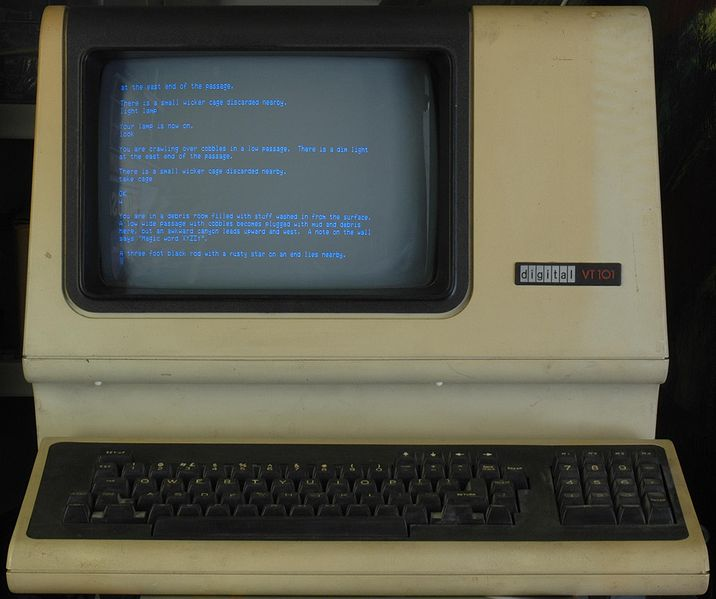
\includegraphics[width=1\textwidth]{figs/vt100}\\ 
        Terminal vt100 
      \end{center}        
    \end{column}
  \end{columns}

\end{frame}



\begin{frame}
      \frametitle{El terminal} 
      \begin{center}
        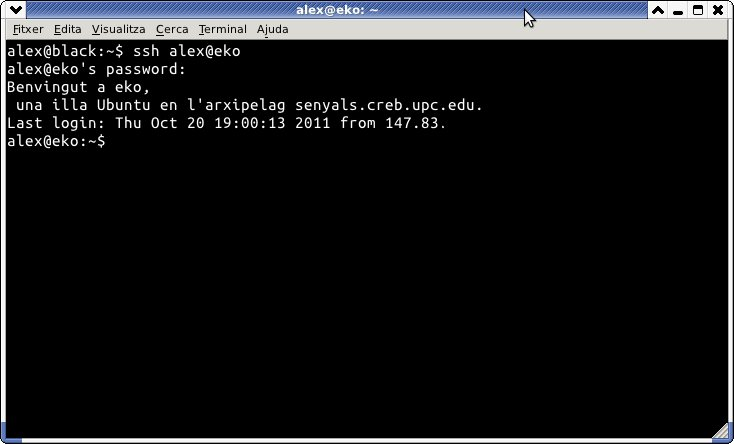
\includegraphics[width=1\textwidth]{figs/terminal} \\
      \end{center}
\end{frame}




\subsection{Estructura de un sistema GNU/Linux}



\begin{frame}
  \frametitle{Estructura del Linux}
  \begin{center}
    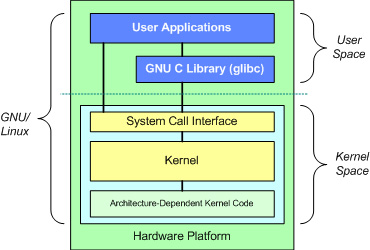
\includegraphics[width=0.9\textwidth]{figs/kernela} \\
  \end{center}
%  \small{  \href{http://ubuntu.com/}{http://ubuntu.com/}}
\end{frame}

\begin{frame}
  \frametitle{Estructura del Linux}
  \begin{center}
    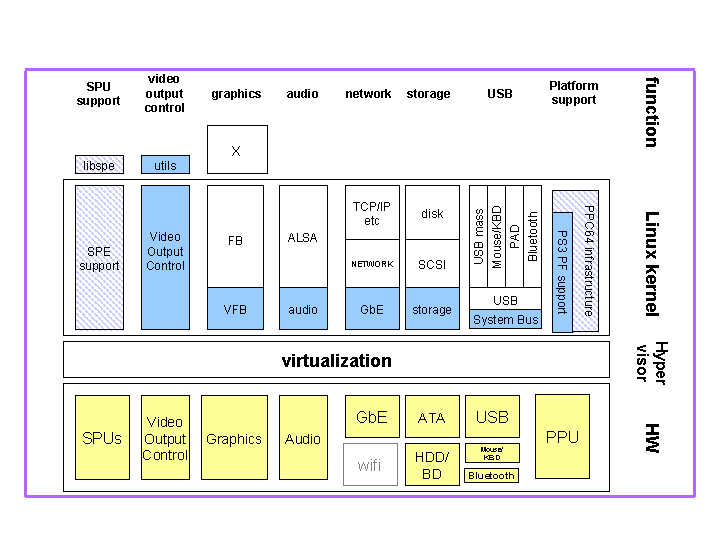
\includegraphics[width=0.9\textwidth]{figs/kernel} \\
  \end{center}
%  \small{  \href{http://ubuntu.com/}{http://ubuntu.com/}}
\end{frame}


\begin{frame}
  \frametitle{Estructura del Linux}
  \begin{center}
    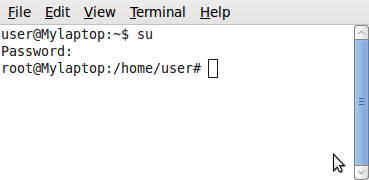
\includegraphics[width=0.9\textwidth]{figs/root-user} \\
  \end{center}
%  \small{  \href{http://ubuntu.com/}{http://ubuntu.com/}}
\end{frame}

\subsection{Sistema de archivos}



\begin{frame}
  \frametitle{Ficheros}
  \begin{block}{Dos cosas importantes a tener en cuenta}
    \begin{enumerate}
    \item<+->  Todo en UNIX son ficheros.
    \item<+->  Todo fichero pertenece a un usuario y a un grupo. 
    \end{enumerate}
  \end{block}
\end{frame}


\begin{frame}
  \frametitle{Sistema d'arxius}
  \begin{itemize}
  \item Los ficheros en UNIX estan almacenados en estructura
    jerárquica, en forma de árbol con una sola raiz. 
  \item Cada nodo ``intermedio'' son directorios.
  \item Cada nodo ``hoja'' son ficheros.
  \end{itemize}
  
  \begin{center}
    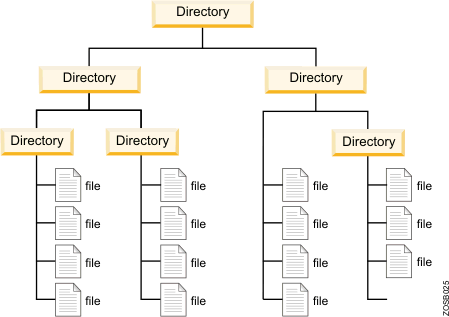
\includegraphics[width=0.7\textwidth]{figs/filesystema} 
  \end{center} 
\end{frame}




\begin{frame}
  \frametitle{Sistema d'arxius}
      \begin{center}
        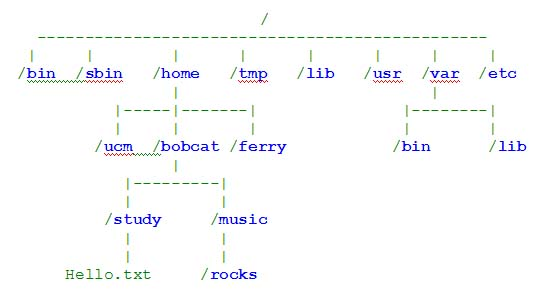
\includegraphics[width=1\textwidth]{figs/filesystemb} 
      \end{center} 
\end{frame}



\begin{frame}
  \frametitle{Sistema de archivos, \emph{pathnames}}
  
      \begin{center}
        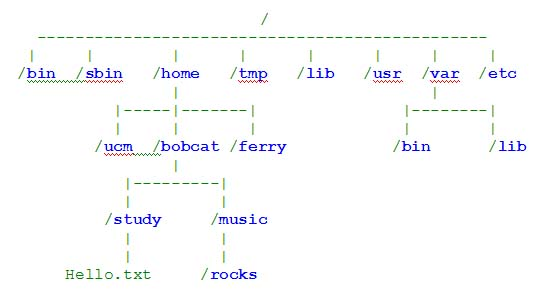
\includegraphics[width=1\textwidth]{figs/filesystemb} 
      \end{center} 
      \begin{itemize}
      \item El camino per acceder a un recuro se denomina \emph{pathname}
      \item e.g. \emph{/home/bobcat/study/Hello.txt}
      \end{itemize}
\end{frame}




\begin{frame}
  \frametitle{Sistema  de archivos, \emph{current pathname}}
  
      \begin{center}
        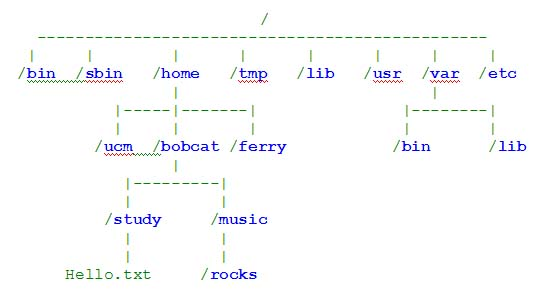
\includegraphics[width=1\textwidth]{figs/filesystemb} 
      \end{center} 
      \begin{itemize}
      \item El \emph{shell} sempre está apuntando en un punto del árbol 
        del sistema de archivos.
      \item Podemos usar \emph{pwd} para obtener el \emph{current pathname}
      \end{itemize}
\end{frame}





\begin{frame}
  \frametitle{Nombres especiales en los fitxers}
  \begin{itemize}
    \item<+-> \emph{/} representa el nodo raiz, o \emph{root directory}.
    \item<+-> \emph{.} representa el directorio actual.
    \item<+-> \emph{..} representa el directorio anterior.
    \item<+-> \emph{$\sim$} representa el directorio del usuario en
      curso. Este  directorio es diferente para cada usuario.
  \end{itemize}
\end{frame}

\begin{frame}
  \frametitle{Ubicacions especials de fitxers}
  \begin{itemize}
    \item<+-> \emph{/home} directorio donde estan todos los directorios
      \emph{home} para cada usuario. Depende de la variante del sistema operativo (e.g. en
      OS X es \emph{ /Users/})
    \item<+-> \emph{/bin} i \emph{/usr/bin}  comandos del sistema
    \item<+->  \emph{/sbin} i \emph{/usr/sbin}  comandos de administración del sistema
    \item<+-> \emph{/etc} directorio con las configuraciones del sistema que afectan a todos los usuarios.
    \item<+-> \emph{/var} varios directorios per usos diferentes
      \begin{itemize}
      \item<+-> \emph{/var/log} contiene archivos que monitorizan la
        actividad del sistema. (actividad de apache, dispositivos,
        red, autorizaciones, ataques al sistema, etc).
      \item<+-> \emph{/var/tmp} y \emph{/tmp} contienen archivos temporales.
      \item<+-> \emph{/var/spool} contiene varios \emph{spools} (carretes o
        bobinas),
        e.g. \emph{cups},    \emph{fax},     \emph{mqueue} y otras.  
      \end{itemize}
    \item<+-> \emph{/dev} contiene fitcheros que representan dispositivos.
    \item<+-> \emph{/proc} conté ficheros especiales, relacionados con el
      sistema.
 \end{itemize}
\end{frame}


\begin{frame}
  \frametitle{Estructura del Linux}
  \begin{center}
    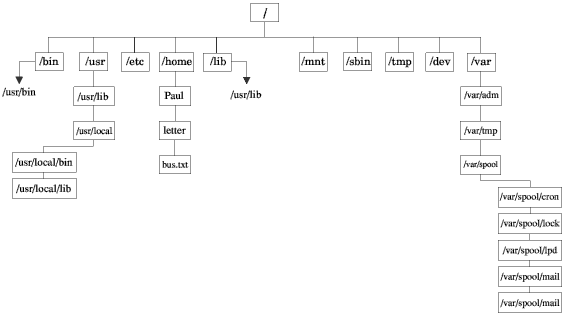
\includegraphics[width=0.9\textwidth]{figs/filesystem} \\
  \end{center}
%  \small{  \href{http://ubuntu.com/}{http://ubuntu.com/}}
\end{frame}


\section{Comandos UNIX útiles}

\begin{frame}
  \frametitle{Comandos UNIX útiles}
  \begin{itemize}
  \item<+-> \emph{cp fuente destino} copia el fichero de fuente a
    destino. Con el  modificador \emph{-r} podemos copiar recursivamente.
  \item<+-> \emph{mv fuente destino } mueve el fichero  o directorio de fuente
    a destino.
  \item<+-> \emph{rm fichero} borra el fichero (\emph{-r}).
    \item<+-> \emph{mkdir directorio} crea un directorio.
    \item<+-> \emph{rmdir directorio} borra un directorio.
  \end{itemize}
\end{frame}






\subsection{Usuarios y Permisos}



\begin{frame}
  \frametitle{Usuaris}
  \begin{itemize}
  \item<+-> Todo en UNIX (persona o programas) que usen el sistema operativo lo hacen mediante un \emph{usuario}.
  \item<+-> El sistema contempla diferentes usuarios, con diferentes privilegios. Existen usuarios especiales:
  \item<+-> \emph{root}: Todo  sistema UNIX tiene un usuario root
    \begin{itemize}
    \item Permite acceder a todos los ficheros del sistema (y por tanto todos los dispositivos)
    \item Tiene su \emph{home} en \emph{/root}.
    \item En ubuntu, no tiene \emph{password} asignado en una instalación estándar, pero realiza las tareas administrativas como 
      \emph{root} mediante \emph{sudo} (Administración de programes (instalación).
    \item \$ - \#
    \end{itemize}
\item<+-> \emph{www-data}: Servidor 
  web.
  \begin{itemize}
  \item Tiene el  \emph{home} en  \emph{/var/www}, que es donde se ubican las páginas web.
  \end{itemize}
  \end{itemize}
\end{frame}



\begin{frame}
  \frametitle{ ls -l}
    \begin{center}
    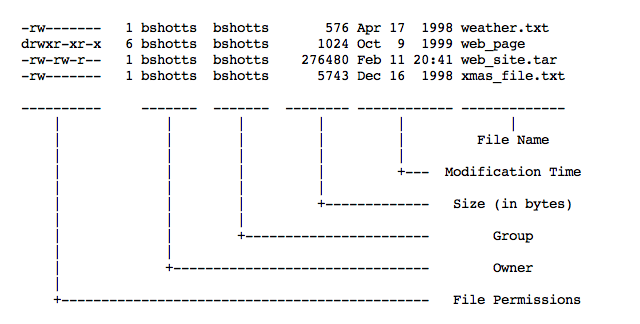
\includegraphics[width=1\textwidth]{figs/lsl} 
  \end{center} 
\end{frame}

\begin{frame}
  \frametitle{Entendiendo ls -l}
  \begin{itemize}
  \item FileName: Nombre del fichero
  \item Modification Time: Fecha última modificación
  \item Size: Tamaño en \emph{bytes}
  \item Group: Grupo propietario 
  \item Owner: Usuario Propietario 
  \item File Permissions: Una representación de los permisos. 
  \end{itemize}
\end{frame}




\begin{frame}
  \frametitle{Permisos en UNIX}
    \begin{center}
    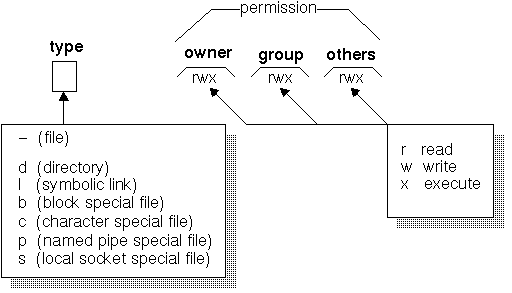
\includegraphics[width=1\textwidth]{figs/permissions} 
  \end{center} 
\end{frame}


\begin{frame}
  \frametitle{Permisos en UNIX}
    \begin{center}
    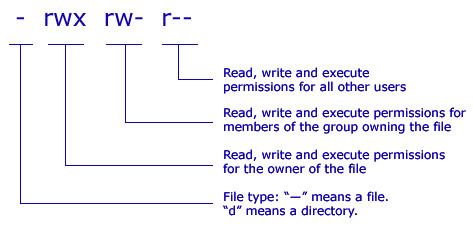
\includegraphics[width=1\textwidth]{figs/permissions0} 
  \end{center} 
\end{frame}


\begin{frame}
  \frametitle{Permisos en UNIX}
    \begin{center}
    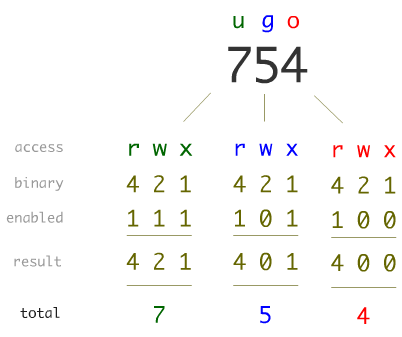
\includegraphics[width=0.8\textwidth]{figs/permissions1} 
  \end{center} 
\end{frame}




\begin{frame}
  \frametitle{Modificando Permisos: chmod}
  \begin{block}{}
    \begin{itemize}
    \item<+-> \emph{chmod 600 test.txt} Modifica todos los permisos
      según un  código binari.
    \item<+-> \emph{chmod o+r test.txt} Modifica los permisos de \emph{others}.
    \item<+->\emph{ chmod o-r test.txt} Deshabilita el bit de lectura
      para \emph{others}
    \item<+-> \emph{chmod g+w test.txt} Habilita el bit de escritura
      para el grupo.
    \item<+-> \emph{chmod u+x test.txt} Habilitat el bit de ejecución
      para el usuario.
    \end{itemize}
  \end{block}
(*) Podeis ver los cambios mediante \emph{ls -l test.txt}. Podeis crear un archivo mediante un editor de texto o \emph{touch}. 
\end{frame}


\begin{frame}
  \frametitle{Modificar el propietario de un archivo o directorio}
  
  La orden chown altera la propiedad de un fichero
  \begin{block}{chown}
    chown alex logfile.txt
  \end{block}
  Hace que la propiedad de \emph{ logfile.txt} pase al usuario  \emph{alex}.\\

(*) Recordad que podeis ver los cambios con \emph{ls -l test.txt}

\end{frame}



\subsection{Gestión de usuarios (vía terminal)}

\begin{frame}
  \frametitle{Añadir y borrar usuarios}
  \begin{block}{Añadir un usuario}
    adduser username
  \end{block}
 \pause \begin{block}{Borrar un usuario}
    deluser username
  \end{block}
\end{frame}



\begin{frame}
  \frametitle{Añadir y borrar grupos}
  \begin{block}{Añadir un grupo}
    addgroup username
  \end{block}
 \pause \begin{block}{Borrar un grupo}
    delgroup username
  \end{block}
\end{frame}



\begin{frame}
  \frametitle{Añadir un usuario a un grupo}
  \begin{block}{}
    adduser username groupname
  \end{block}
\end{frame}


\begin{frame}
  \frametitle{Gestió d'usuaris a Ubuntu (GUI)}
  \begin{columns}
    \begin{column}{0.5\textwidth}
      \begin{itemize}
      \item Ubuntu contiene una herramienta gráfica para la gestión de usuarios
      \item Permite la gestión fácil de usuarios y grupos. 
      \end{itemize}
    \end{column}
    \begin{column}{0.5\textwidth}
      \begin{center}
        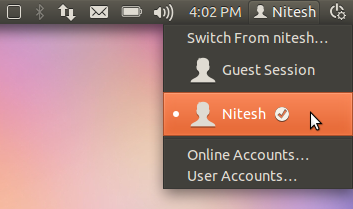
\includegraphics[width=0.5\columnwidth]{figs/ubntuusermenu}
      \end{center}

      \begin{center}
        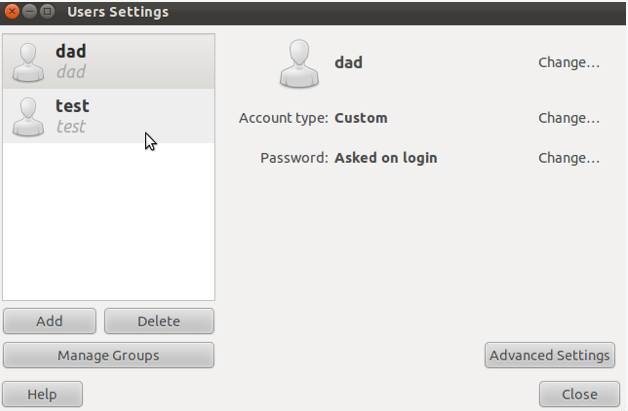
\includegraphics[width=0.7\columnwidth]{figs/users}
      \end{center}
    \end{column}

  \end{columns}

\end{frame}
 


\subsection{Ejecutando  tareas como  administrador}

\begin{frame}
  \frametitle{Quién puede ejecutar tareas como administrador (ubuntu)}
  \begin{itemize}
  \item<+-> El usuario \emph{root} no tiene contraseña.
  \item<+-> En los sistemas \emph{ubuntu} los usuarios que pertenecen al grupo  \emph{admin} pueden ejecutar tareas como  administrador.
  \item<+-> Se escalan privilegios mediante \emph{sudo}.
  \item<+-> Ejemplo \emph{sudo visudo } edita el fichero que define
    quién puede escalar privilegios. (Intentad encontral la entrada que determinal que el grupo \emph{admin} puede utilizar \emph{sudo})
  \end{itemize}
\end{frame}


\subsection{Instalando programas}

\begin{frame}
  \frametitle{Desde la linea de comandos}
  \begin{block}{apt-get (ubuntu)}
    Necesitamos saber el nombre del \emph{paquete}, entonces 
     \emph{apt-get}.
  \end{block}
\pause  \begin{block}{Actualización de un sistema}
  \emph{apt-get update}\\
  \emph{apt-get upgrade}
  \end{block}
\end{frame}




\begin{frame}
  \frametitle{Herramientas de actualitzación (GUI)}
  \begin{block}{synaptic}
    \emph{synaptic} es un programa para ayudarnos en la administración de programas. 
  \end{block}

 \begin{center}
    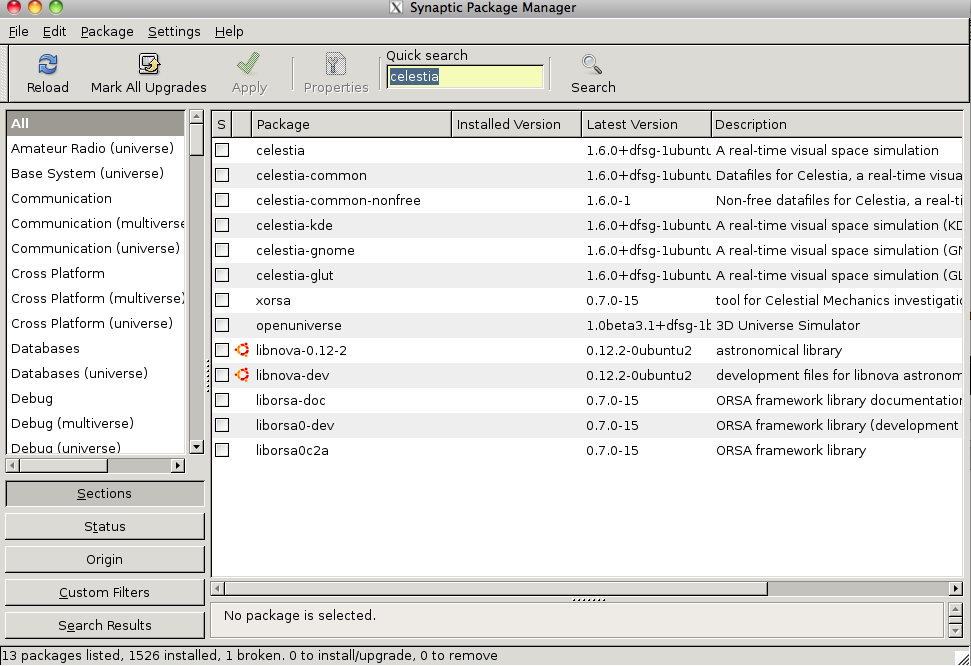
\includegraphics[width=0.7\textwidth]{figs/synaptic} 
  \end{center} 
\end{frame}



\begin{frame}
  \frametitle{Ejercicio}
  \begin{block}{}
    \begin{itemize}
    \item<+-> Buscad e instalad los components ipython y ipython-notebook.
    \item<+-> Buscad e instalad el editor para pyhton \emph{spyder}
    \end{itemize}
  \end{block}
\end{frame}





\begin{frame}
  \frametitle{Fin de la Parte I }
  \begin{center}
    \centering 
\includegraphics[width=0.5\linewidth]{figs/question_mark}
  \end{center}
\end{frame}
\end{document}

